\chapter{AdaptaMaterialEscolar2.0}
\label{cap:AdaptaMaterialEscolar2.0}
En este capítulo explicaremos la obtención de requisitos y su priorización en la Sección \ref{cap:requisitos}. También se describirá la iteración competitiva para el diseño de la aplicación en la Sección \ref{disenyoDeLaAplicacion}.

\section{Requisitos}
\label{cap:requisitos}
En esta sección se explicara la tabla de requisitos.

Lo primero que realizamos fue analizar la memoria anterior extrayendo las funcionalidades que faltan por implementar y las propuestas por los profesores. Para la priorización de las funcionalidades utilizamos el coste y la importancia, usando la siguiente formula: prioridad = coste * importancia. Para el primero se definió un rango del 5 al 1 donde el 5 es el menor coste y 1 es el mayor. Para la importancia se estableció un rango del 1 al 5 en el cual el 1 es la menor importancia y el 5 la mayor. A continuación, se muestran las funciones priorizadas en la Tabla \ref{tabla_priorizacion}.
\\
\begin{table}
    \begin{tabular}{|l|c|c|c|}
    \hline
    \multicolumn{1}{|c|}{Funciones} &
      Coste &
      Importancia &
      Prioridad \\ \hline
    \begin{tabular}[c]{@{}l@{}}Añadir encabezado al texto\\ (como word lista de estilos de encabezado).\end{tabular} &
      5 &
      5 &
      25 \\ \hline
    Generar un resumen a partir de un texto. &
      5 &
      5 &
      25 \\ \hline
    \begin{tabular}[c]{@{}l@{}}Exportar el documento a formato Word \\ para hacer modificaciones.\end{tabular} &
      5 &
      5 &
      25 \\ \hline
    \begin{tabular}[c]{@{}l@{}}Añadir un pictotraductor como \\ funcionalidad.\end{tabular} &
      5 &
      4 &
      20 \\ \hline
    \begin{tabular}[c]{@{}l@{}}Ejercicios de relacionar contenido \\ mediante flechas.\end{tabular} &
      5 &
      3 &
      15 \\ \hline
    \begin{tabular}[c]{@{}l@{}}Añadir imágenes buscando una palabra \\ en bases de datos de imágenes libres.\end{tabular} &
      3 &
      4 &
      12 \\ \hline
    Añadir un tipo de fuente escolar. &
      5 &
      2 &
      10 \\ \hline
    Sustituir una palabra por una imagen. &
      2 &
      4 &
      8 \\ \hline
    \begin{tabular}[c]{@{}l@{}}Añadir una leyenda de colores con la \\ categoría de cada tipo.\end{tabular} &
      4 &
      2 &
      8 \\ \hline
    \begin{tabular}[c]{@{}l@{}}Añadir ejercicios para ejercicios de \\ cálculo con fórmulas con huecos a\\ rellenar por el alumno.\end{tabular} &
      4 &
      2 &
      8 \\ \hline
    \begin{tabular}[c]{@{}l@{}}Añadir ejercicios con espacio para \\ dibujar.\end{tabular} &
      5 &
      1 &
      5 \\ \hline
    \begin{tabular}[c]{@{}l@{}}Añadir leyenda de colores para el \\ tema de cada asignatura(color borde \\ personalizar colores).\end{tabular} &
      4 &
      1 &
      4 \\ \hline
    \begin{tabular}[c]{@{}l@{}}Añadir ejercicios de matemáticas con \\ cuadrícula para escribir los números.\end{tabular} &
      3 &
      1 &
      3 \\ \hline
    \begin{tabular}[c]{@{}l@{}}Añadir la alternativa de añadir doble \\ pauta, en vez de renglones de una \\ única línea, para determinar el \\ tamaño de la letra del alumno.\end{tabular} &
      3 &
      1 &
      3 \\ \hline
    \begin{tabular}[c]{@{}l@{}}Crear tablas que organicen el temario \\ y/o las actividades, seleccionando \\ contenido.\end{tabular} &
      1 &
      3 &
      3 \\ \hline
    \begin{tabular}[c]{@{}l@{}}Crear esquemas que faciliten la \\ visualización.\end{tabular} &
      1 &
      3 &
      3 \\ \hline
    \begin{tabular}[c]{@{}l@{}}Ejercicios de completar los espacios \\ en blanco en tablas y esquemas.\end{tabular} &
      1 &
      2 &
      2 \\ \hline
    \begin{tabular}[c]{@{}l@{}}Estandarizar formato para títulos e \\ índices del temario.\end{tabular} &
      1 &
      1 &
      1 \\ \hline
    \begin{tabular}[c]{@{}l@{}}Crear una herramienta de recorte de \\ imágenes para el texto original.\end{tabular} &
      1 &
      1 &
      1 \\ \hline
    \begin{tabular}[c]{@{}l@{}}Enumerar ejercicios de forma \\ automática.\end{tabular} &
      1 &
      1 &
      1 \\ \hline
    \end{tabular}
    \caption{Lista de priorización}
    \label{tabla_priorizacion}
\end{table}
\section{Diseño de la apliación}
\label{disenyoDeLaAplicacion}
Para el diseño de la aplicación web hemos realizado una iteración competitiva. Cada integrante del grupo ha proporcionado un diseño de la apliación como se muestra en las figuras \ref{IteracionCompetitiva1}, \ref{IteracionCompetitiva2}, \ref{IteracionCompetitiva3} y \ref{IteracionCompetitiva4}.
Una vez que cada integrante ha explicado su diseño, hemos cogido lo mejor de cada uno quedando la aplicación de la siguiente manera \ref{diseño_final}.


\begin{figure}[ht!]
    \centering
    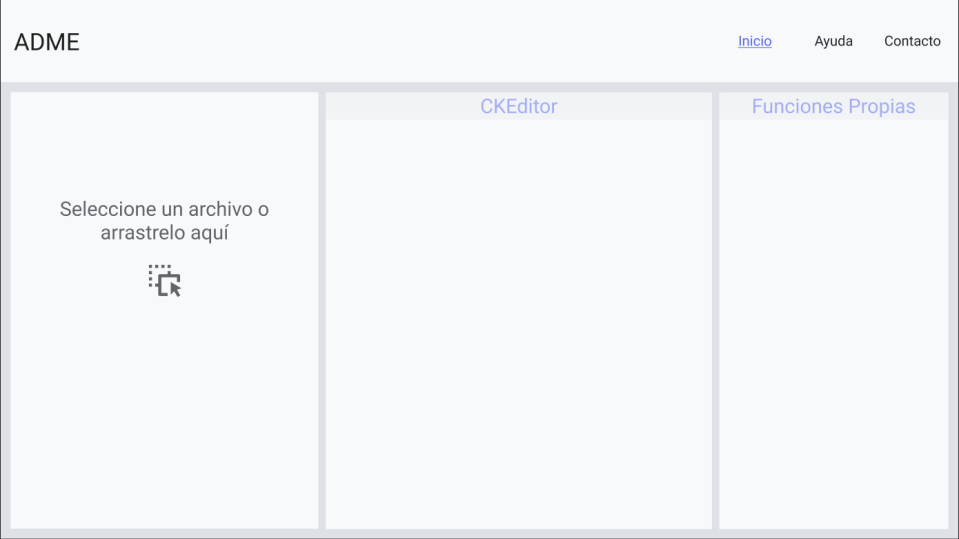
\includegraphics[scale=0.3]{IteracionCompetitiva1}
    \caption{Diseño aplicación iteración competitiva 1.}
    \label{IteracionCompetitiva1}
\end{figure}
\begin{figure}[ht!]
    \centering
    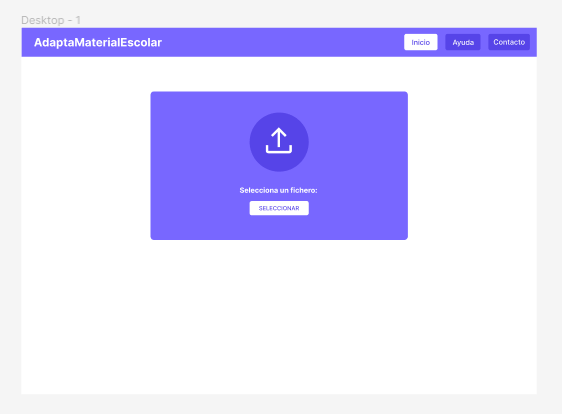
\includegraphics[scale=0.5]{IteracionCompetitiva2}
    \caption{Diseño aplicación iteración competitiva 2.}
    \label{IteracionCompetitiva2}
\end{figure}
\begin{figure}[ht!]
    \centering
    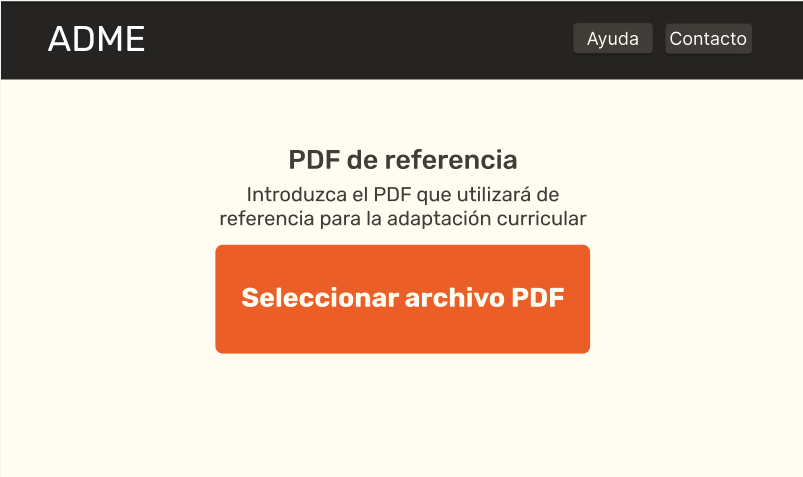
\includegraphics[scale=0.5]{IteracionCompetitiva3}
    \caption{Diseño aplicación iteración competitiva 3.}
    \label{IteracionCompetitiva3}
\end{figure}
\begin{figure}[ht!]
    \centering
    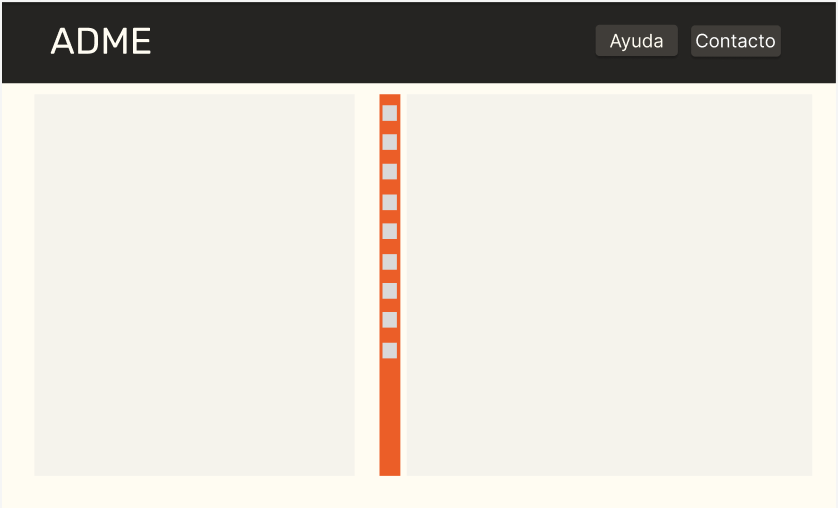
\includegraphics[scale=0.5]{IteracionCompetitiva4}
    \caption{Diseño aplicación iteración competitiva 4.}
    \label{IteracionCompetitiva4}
\end{figure}
\begin{figure}[ht!]
  \centering
  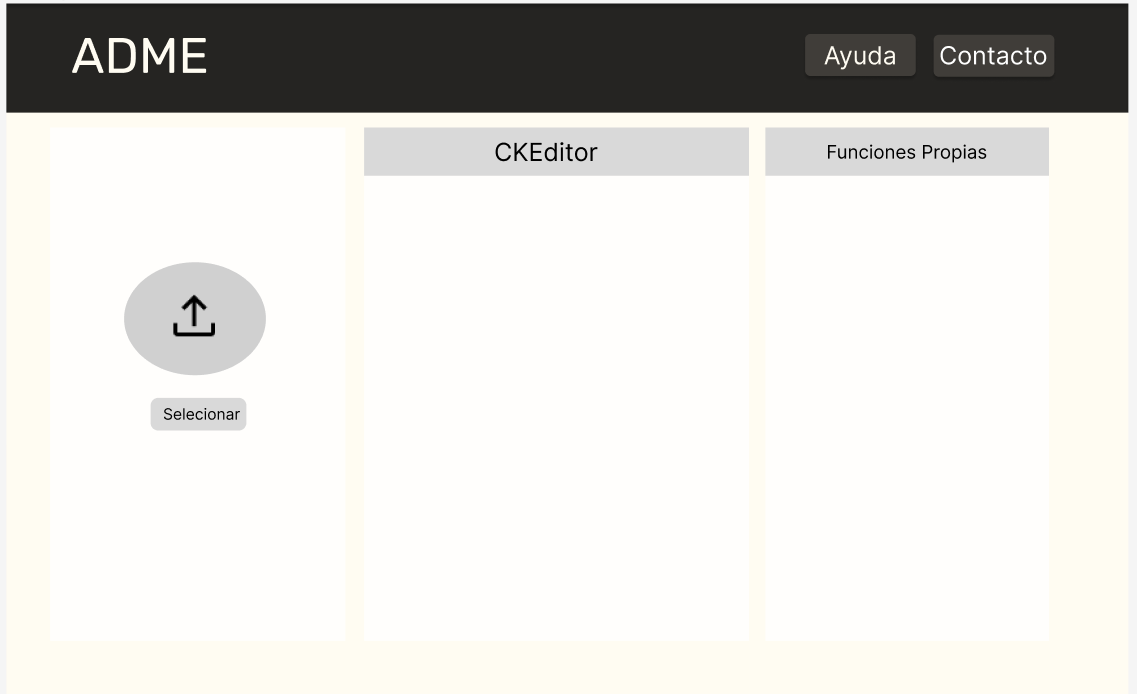
\includegraphics[scale=0.3]{Diseño Final}
  \caption{Diseño final apliación.}
  \label{diseño_final}
\end{figure}
